\documentclass[../documentation.tex]{subfiles}
 
\begin{document}
\section{A megfogó vezérlése}
\subsection{A vezérlés hardveres kialakítása}
Ahhoz hogy a megfogót (grippert) a robotvezérlőn futó programból lehessen irányítani, több kiegészítő eszközre is szükség van a gripperen és a vezérlőegységén kívül. Többféle konstrukcióval is el lehet érni ezt a célt. A projekt során használt összeállítás elemei (\ref{fig:grippersetup}):
\begin{itemize}
	\item \textbf{Megfogó (gripper):} párhuzamosan mozgó, két pofájú, elektromos megfogó; pontos típusa: SCHUNK MEG 50 EC\cite{grippermanual}.
	\item \textbf{Grippervezérlő:} a megfogóhoz tervezett vezérlő; pontos típusa: SCHUNK Controller MEG EC\cite{grippermanual}
	\item \textbf{Analóg és digitális I/O modulok\footnote{I/O (\angol{(Input/Output)}: bemeneti és kimeneti modulok}:} a robotvezérlő ezen modulok segítségével tudja irányítani a grippervezérlőt. A felhasznált eszközök Beckhoff gyártmányúak. Pontos tipusaik:
	\begin{itemize}
		\item EL1809: 16 csatornás, digitális bemeneti modul\footnote{https://www.beckhoff.com/english.asp?ethercat/el1809.htm}
		\item EL2809: 16 csatornás, digitális kimeneti modul\footnote{https://www.beckhoff.com/english.asp?ethercat/el2809.htm}
		\item EL3002: 2 csatornás, analóg bemeneti modul\footnote{https://www.beckhoff.hu/english.asp?ethercat/el3002.htm}
		\item EL4032: 2 csatornás, analóg kimeneti modul\footnote{https://www.beckhoff.com/english.asp?ethercat/el4032.htm}
	\end{itemize}
	\item \textbf{EtherCAT\footnote{Általános ismertető az EtherCAT-ről: https://en.wikipedia.org/wiki/EtherCAT} Coupler:} az I/O modulok az ú.n. E-bus-on keresztül kommunikálnak. Ahhoz hogy a robotvezérlőhöz lehessen kötni az E-bus-t, EtherCAT Coupler-re van szükség. Pontos tipusa: Beckhoff EK1100\footnote{https://www.beckhoff.com/english.asp?ethercat/ek1100.htm}.
	\item \textbf{Tápegység:} a fentebb felsorolt eszközök mindegyike 24 V megtáplálást igényel, ezt a projekt során egy Siemens tápegység szolgáltatja.
\end{itemize}

\begin{figure}
\centering
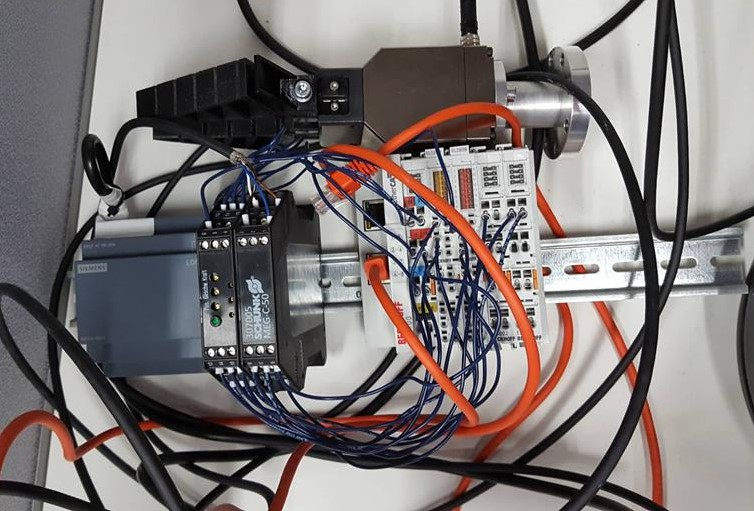
\includegraphics[scale=0.11]{grippersetup}
\caption{Kép a megfogóhoz tartozó konstrukcióról}
\label{fig:grippersetup}
\end{figure}

\subsection{A megfogó szoftveres konfigurációja}
KUKA SunriseOS esetén (és általánosságban a KUKA robotok esetén) a különböző bemeneti, kimeneti és kommunikációs csatornák kezelésére I/O konfigurációs fájl generálására van szükség. Ezeket a fájlokat a KUKA WorkVisual nevű program segítségével lehet létrehozni és szerkeszteni. Adott KUKA SunriseOS-hez meghatározott a kompatibilis Sunrise Workbench verzió (ebben a programban a legegyszerűbb a robotvezérlőn futó program megírása, feltöltése). Adott Sunrise Workbench verzóval kompatibilis WorkVisual verzóra vonatkozó információkat a Sunrise Workbench-et megnyitva a Help->Sunrise.OS Release Notes menüpont alatt találunk. A szakdolgozathoz felhasznált szoftverek és környezet:
\begin{itemize}
	\item SunriseOS 16
	\item Work Visual 5.0.5 build600
	\item Windows 10 a PC-n
\end{itemize}

A megfelelő IOConfig elkészítéséhez az alábbi lépések szükségesek:
\begin{enumerate}
	\item Ahhoz hogy a WorkVisual verziót összekössük a Sunrise Workbench-csel importálni kell a Workbench-hez tartozó Sunrise.kop fájl a WorkVisual-ba. Ez a fájl a telepített Workbench verzióhoz tartozó mappán belül a `WorkVisual AddOn' nevű almappában található. Az importálás menete: WorkVisual->Extras->Option package management->Install... gomb. A felugró ablakban lehet kiválasztani a megfelelő Sunrise.kop fájlt és telepíteni. Ahhoz hogy az egyes Beckhoff modulokkal lehessen kommunikálni szükség van a `Device description file'-ok importálására. Ezek a fájlok a gyártó oldaláról letölthetőek\footnote{Device description files: https://www.beckhoff.com/english.asp?download/elconfg.htm}. A (XML) fájlok importálásához a WorkVisual->Import / Export->Import device description file lehetőséget kell választani (ezt a műveletet adott eszközön csak egyszer kell elvégezni, új projekt esetén ezt a lépést már ki lehet hagyni). A megfelelő fájlok kiválasztása és importálása után szükség van a DTM Catalog frissítésére (WV->Extras->DTM Catalog Management->Search for installed DTMs). A fájlok használatához a `Known DTMs' részről át kell emelni az elemeket a `Current DTM Catalog' részre (\ref{fig:dtmcatalog}).
	\item A Sunrise Workbench-ben új projekt létrehozása után a projektre jobb egérgomb->New->I/O Configuration. A WorkVisual automatikusan elindul. A projektre jobb egérgombbal kattintva (WV-ban) a `\angol{Set as active controller}' lehetőséget kell választani. A busz struktúrákhoz hozzá kell adni a `KUKA Extension Bus (SYS-X44)' elemet ahhoz, hogy az EtherCAT kommunikációt inicializáljuk a robotvezérlőben. Ehhez adhatjuk hozzá az EK1100 EtherCAT Coupler-t, ami az összeköttetést biztosítja a robotvezérlőben található EtherCAT hálózat és a modulok között (E-bus). Az egyes modulokat ehhez adhatjuk hozzá a programban. \textbf{Fontos:} az egyes fájlokat olyan sorrendben kell hozzáadni, ahogy azok fizikailag kapcsolódnak egymáshoz (\ref{fig:ethercatconfig} ábra).
	\item Ahhoz hogy ezeket a be- és kimeneteket a Sunrise Workbench-ben használni tudjuk szükség van Sunrise I/O Group létrehozására (VW->IO Mapping->Sunrise I/Os->Creates signals at the provider). Az I/O Group-nak tetszőleges nevet adhatunk. Az egyes be- és kimenetek kezeléséhez létrehozhatunk változókat az I/O Group-on belül. A gripper nyitásához és zárásához alapvetően 3 változó deklarálása elegendő\footnote{A gripper nyitásához és zárásához elegendő csak a digitális ki- és bementeket használni, de például a pozíció követéséhez használni kell analóg bemeneti modult, a fogóerő programból történő beállításához pedig analóg kimeneti modult.}), pl.:
	\begin{itemize}
		\item OpenGripper: bool, output, digital
		\item CloseGripper: bool, output, digital
		\item Status: bool, input, digital
	\end{itemize}
Az egyes változókat a kívánt bemenetekkel és kimenetekkel \angol{Drag and drop} módszerrel lehet összerendelni (\ref{fig:signalsmatching}). Megfelelő összekötés esetén a változók mellletti szürke nyilak zölddé változnak.
	\item Az elkészült I/O konfigurációt exportálni kell ahhoz, hogy a Sunrise Workbench-ben használni lehessen (WV->File->Import / Export->\angol{Export I/O Configuration to Sunrise Workbench project}). A Workbench-ben ezek után megjelenik az `src' mappában egy ioAccess nevű csomag. Ezen belül található az IO Group-hoz tartozó osztály (pl.: GripperContolIOGroup.java). Ez tartalmazza a szükséges metódusokat a gripper vezérléséhez, ezeket lehet meghívni a programból.
\end{enumerate}

\begin{figure}[h]
\centering
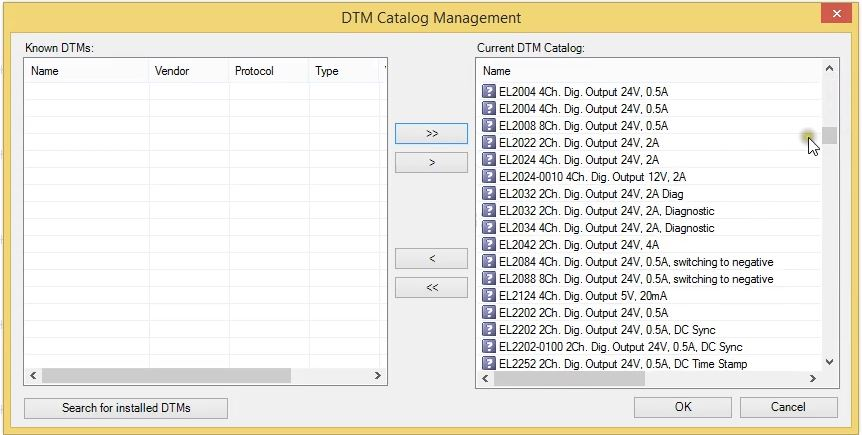
\includegraphics[scale=1]{dtmcatalog}
\caption{Az xml fájlok sikeres beimportálása után láthatjuk a \angol{Device description} fájlokat}
\label{fig:dtmcatalog}
\end{figure}

\begin{figure}[h]
\centering
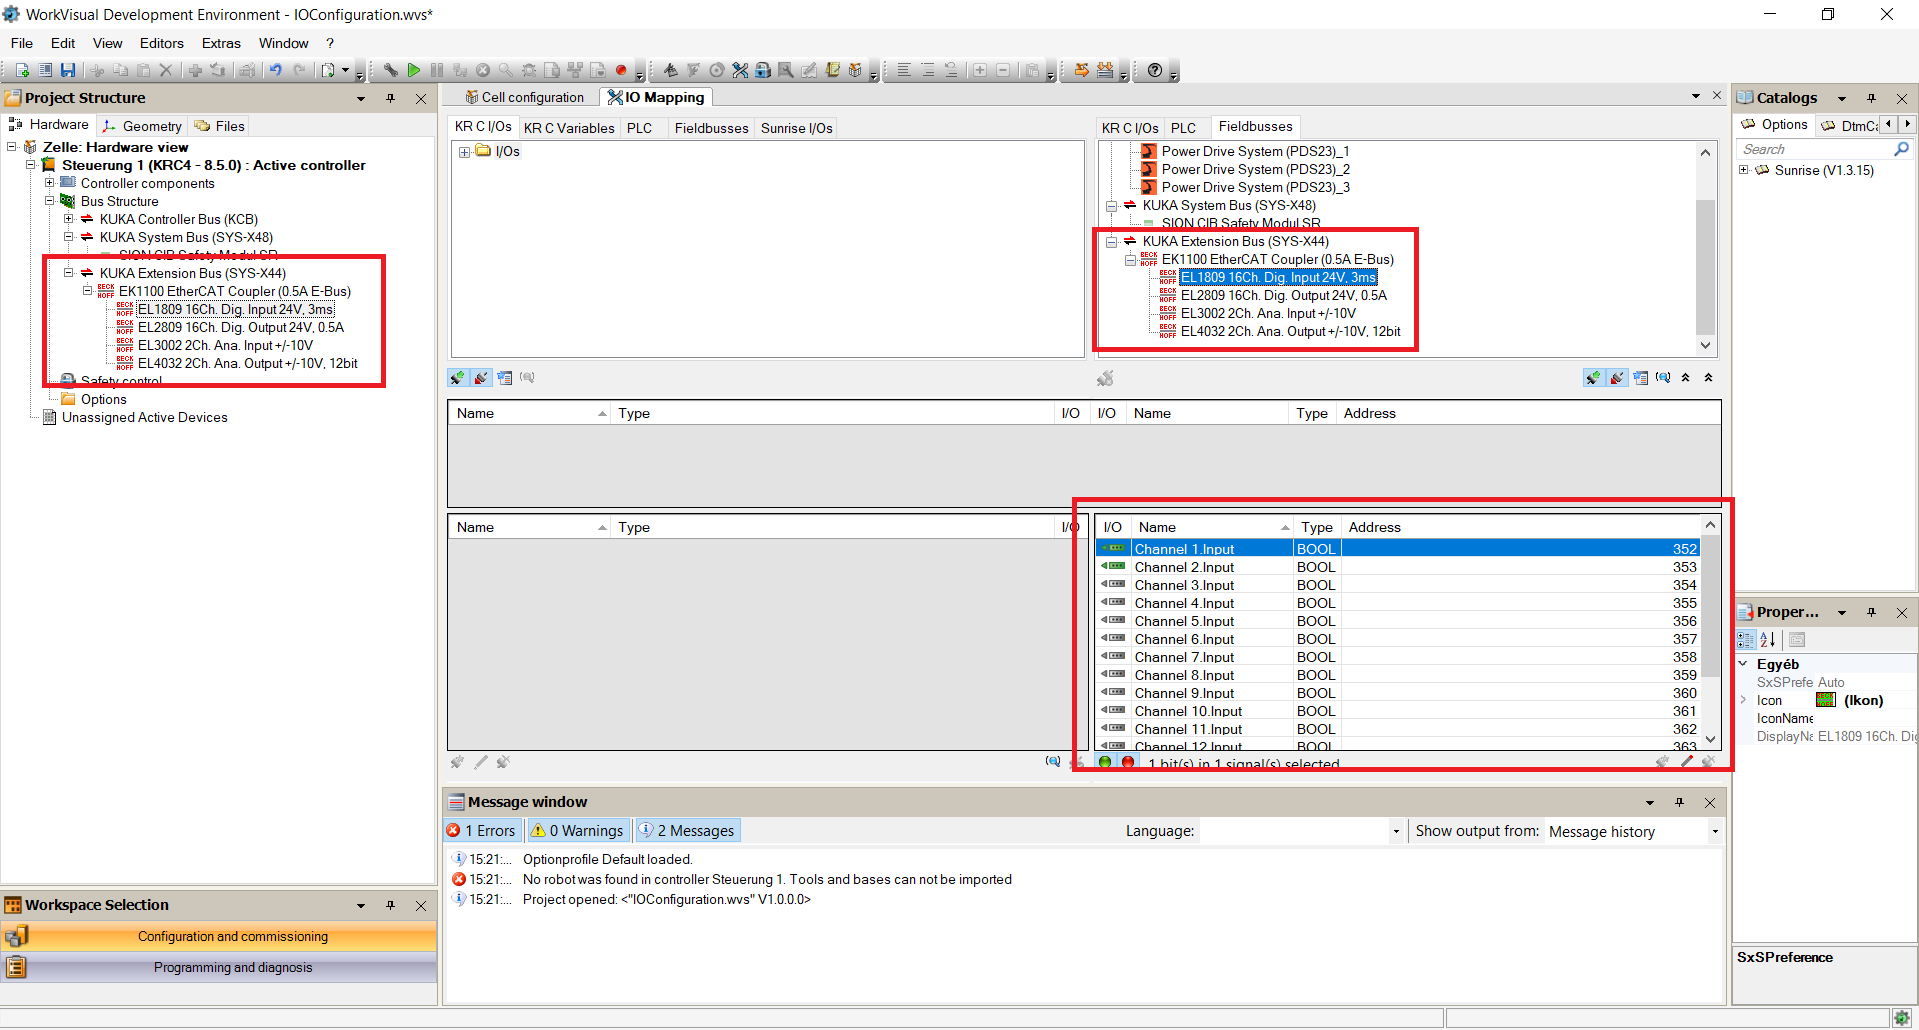
\includegraphics[scale=0.45]{ethercatconfig}
\caption{Az EtherCAT konfiguráció}
\label{fig:ethercatconfig}
\end{figure}

\begin{figure}[h]
\centering
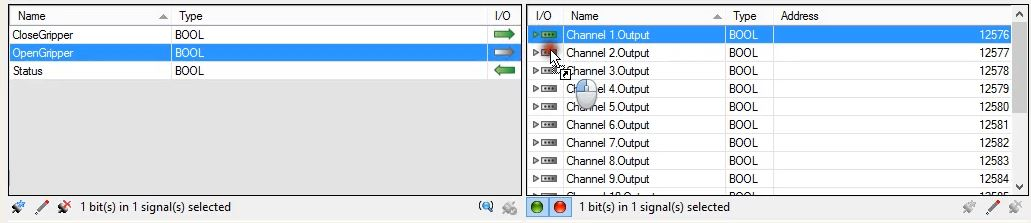
\includegraphics[scale=0.75]{signalsmatching}
\caption{Az I/O változók hozzárendelése a be- és kimenetekhez}
\label{fig:signalsmatching}
\end{figure}

%\clearpage



\end{document}